Following picture is Figure.\ref{Firework}

\begin{figure}[H]
\centering
\includegraphics[width=\linewidth,height=10cm,keepaspectratio]{Figure/Firework.JPG}
\caption{Firework}
\label{Firework}
\end{figure}


\begin{figure}[H]
\centering
\begin{minipage}{.5\linewidth}
  \centering
  \includegraphics[width=.7\linewidth]{light}
  \captionof{figure}{A figure}
  \label{fig:test1}
\end{minipage}%
\begin{minipage}{.5\linewidth}
  \centering
  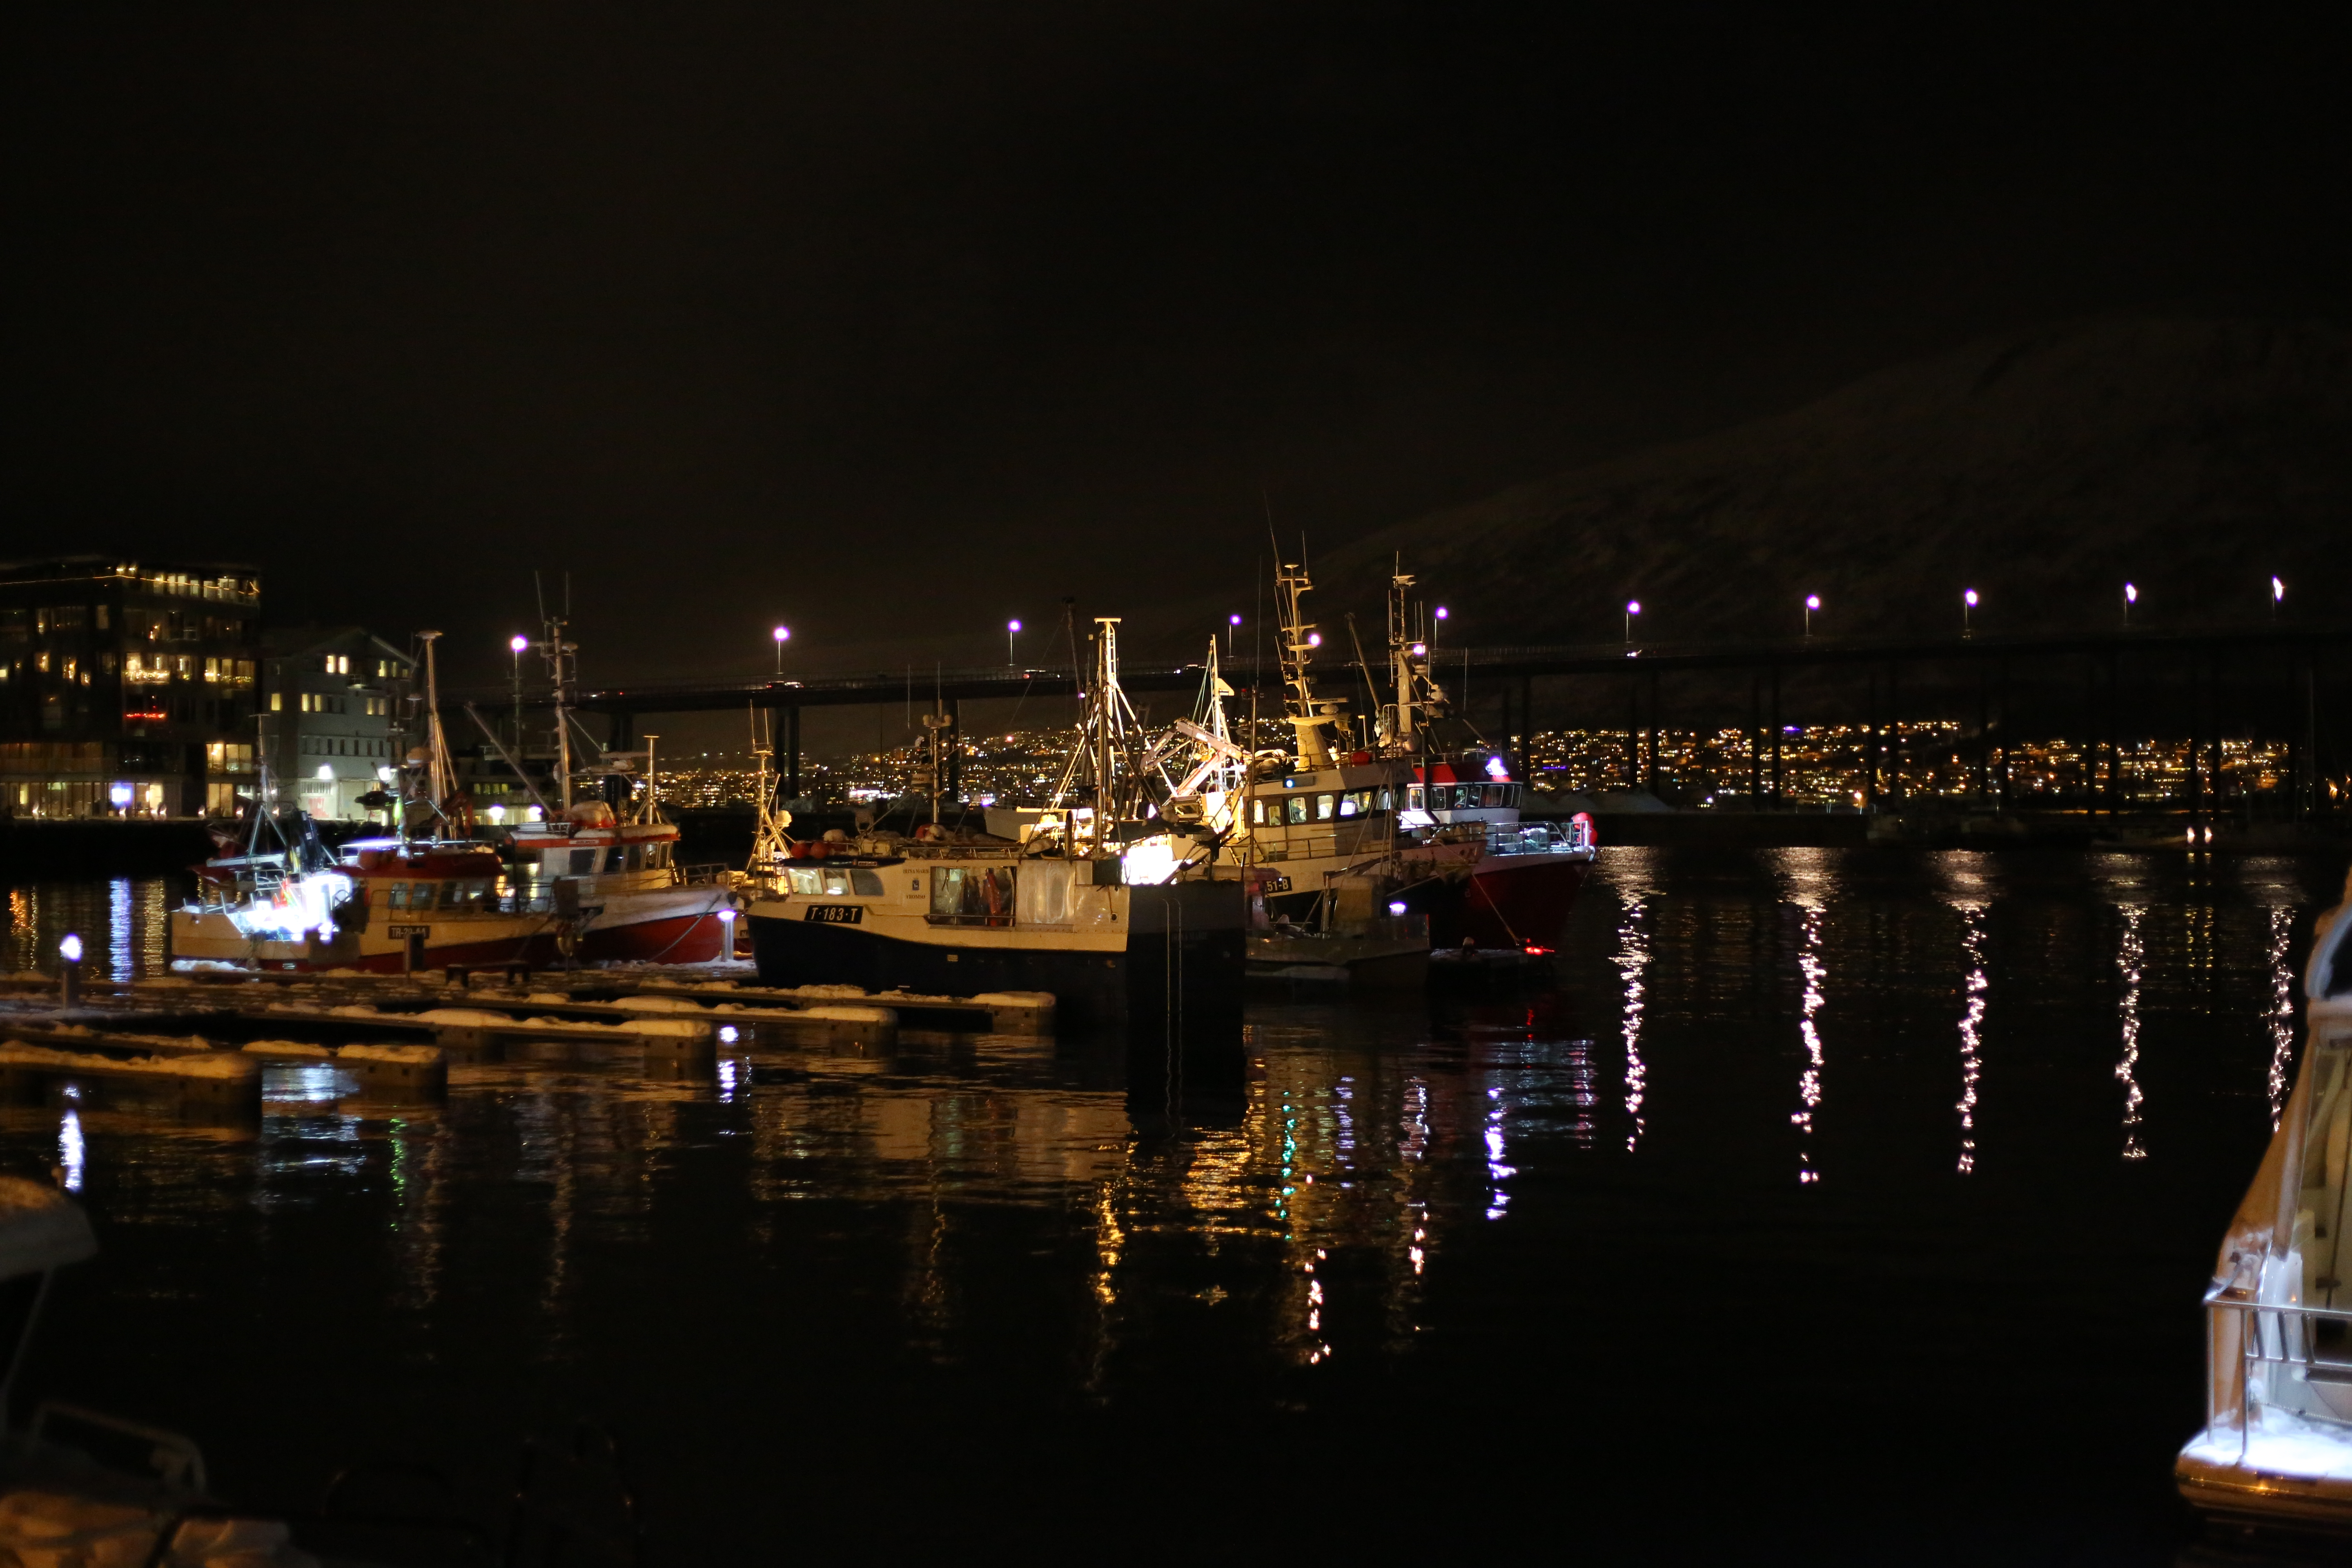
\includegraphics[width=.7\linewidth]{view}
  \captionof{figure}{Another figure}
  \label{fig:test2}
\end{minipage}
\end{figure}


\begin{figure*}[t]
\centering
\begin{tabular}{@{}ccc@{}}
\subfloat[a]{\includegraphics[width=0.3\textwidth]{Firework}} & 
\subfloat[b]{\includegraphics[width=0.3\textwidth]{light}} &
\subfloat[c]{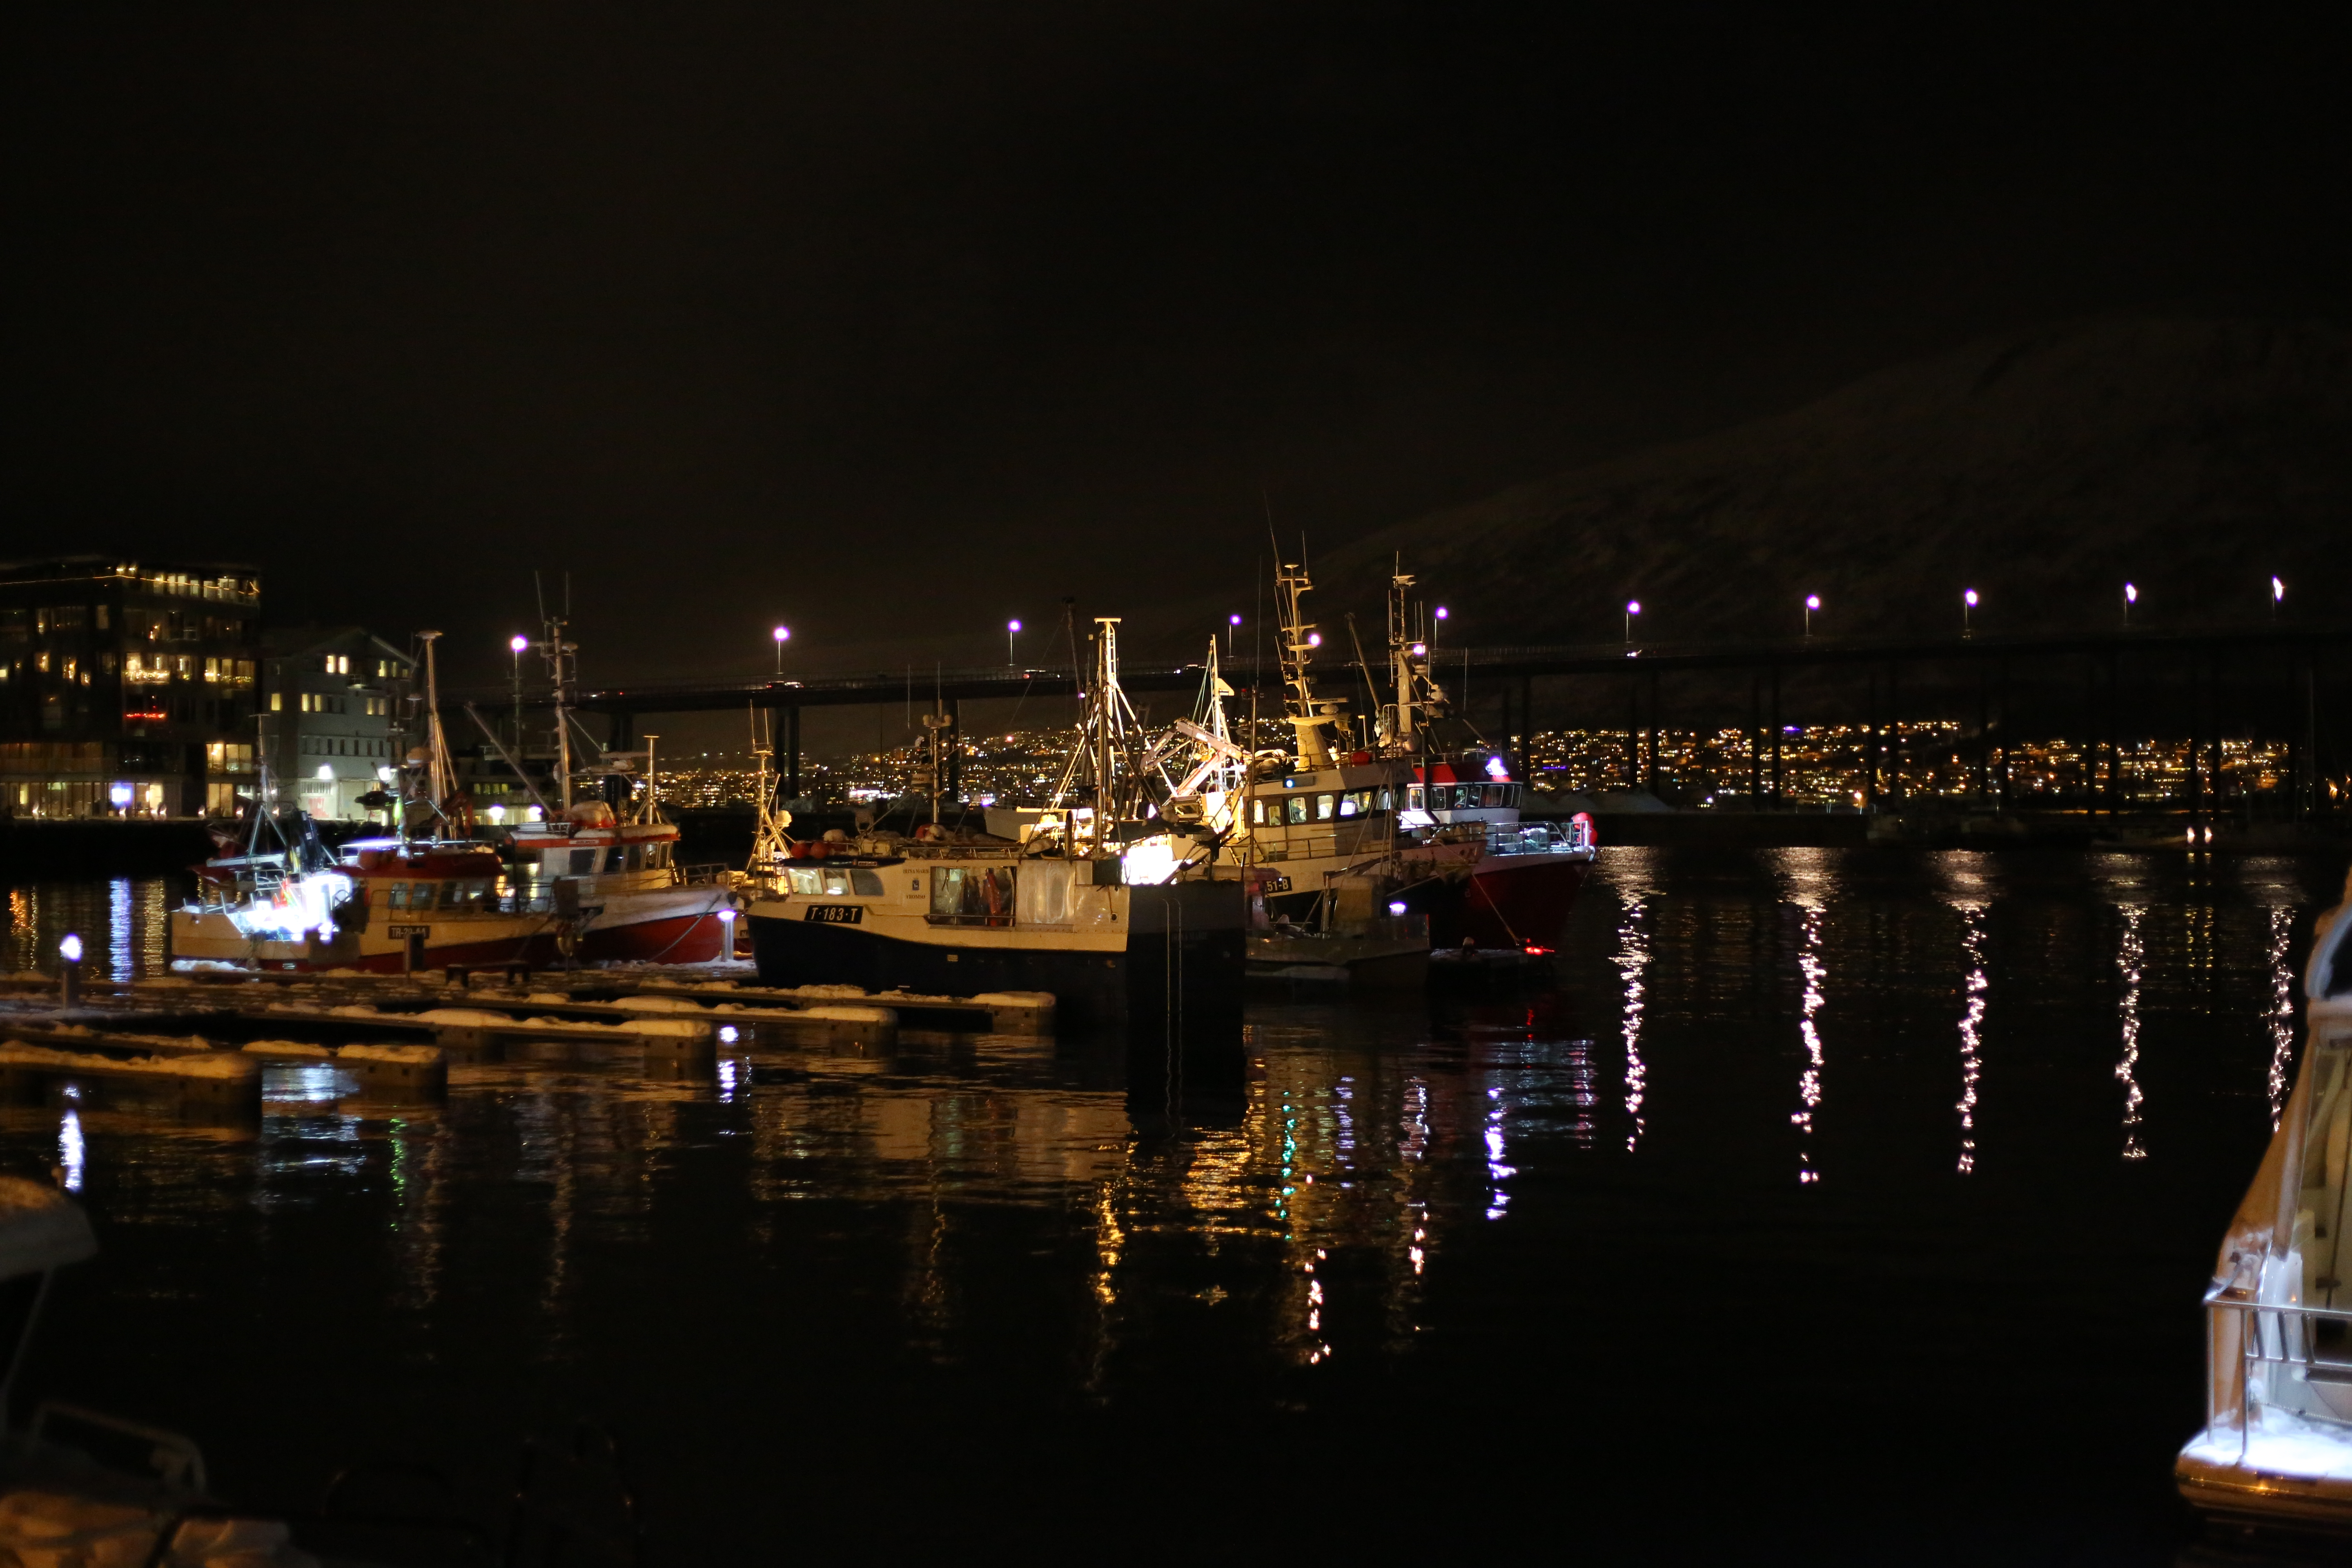
\includegraphics[width=0.3\textwidth]{view}} \\
\end{tabular}
\caption[]{Description}
\label{fig:ABC}
\end{figure*}

